\documentclass{report}
\usepackage[utf8]{inputenc}
\usepackage[pdftex]{graphicx}
\usepackage{tikz}
\usepackage{listings}
\usepackage{color}
\usepackage{float}

\definecolor{javared}{rgb}{0.6,0,0} % for strings
\definecolor{javagreen}{rgb}{0.25,0.5,0.35} % comments
\definecolor{javapurple}{rgb}{0.5,0,0.35} % keywords
\definecolor{javadocblue}{rgb}{0.25,0.35,0.75} % javadoc

\lstset{language=Java,
basicstyle=\ttfamily,
keywordstyle=\color{javapurple}\bfseries,
stringstyle=\color{javared},
commentstyle=\color{javagreen},
morecomment=[s][\color{javadocblue}]{/**}{*/},
numbers=left,
numberstyle=\small\color{black},
stepnumber=1,
numbersep=10pt,
tabsize=4,
showspaces=false,
showstringspaces=false}


\title{FacelookCA - The next generation of Cellular Automata}
\author{Benjamin Chung, Cory Williams,
Hank Zwally}%more
\begin{document}
\maketitle
\tableofcontents
\chapter{Introduction}
FacelookCA is designed to be a fast, efficient, and expandable framework for
Cellular automata. It provides interfaces for both single-threaded and
multi-threaded execution of cellular automata, as well as a expandable rule
framework allowing for nearly infinate varibillity in rules.


To the grader, please note that our sample code includes the contents of the
package org.scubaguy.facelook.automata, as it contains implementations of every
publically facing interface.
\section{Boards}
FacelookCA supports square boards, with each cell reperesented as a 32 bit
integer. 
\section{Rules}
FacelookCA is based around Rules. A Rule is a piece of code that determines what
state a given cell should be in. FacelookCA supports standard MCell notation for
rules, as well as custom code.
\section{Executers}
FacelookCA uses two executers, a single-threaded one, and a multi-threaded one.
The single threaded executer is the executer that you are most likly to use, as
it supports any rule. The multithreaded executer is signifigantly faster, but at
the expense of being much harder to code for. It is reccomended to start with
the single-threaded executer.
\section{GUI}
FacelookCA can display the state of a Cellular Automata using Java Swing,
through a simple interface. In order to display a board, a cell renderer has to be created. The
renderer handles both the display of cells, as well as user input to alter
cells. FacelookCA, by default, includes a two state renderer.
\section{Loaders}
FacelookCA calls file importers Loaders. Loaders are managed by a singleton
instance of a Loader manager, which can automatically load a file into a board.
The framework will eventually include loaders for standard CA format.
\chapter{Getting Started}
To get started with FacelookCA, we will create a simple Conway's game of life
using the framework.


Using the IDE of your choice, create a new project containing a class with a
main function, and make sure that it
works.
\begin{figure}[H]
\begin{lstlisting}
public class GameOfLife {
    public static void main(String[] args) {

    }
}
\end{lstlisting}
\caption{The basics}
\label{code:start}
\end{figure}


We now need to add a reference to the FacelookCA library in the project. I don't
know what IDE you are using, so I can't give specific instructions as to how to
add it to the project. 


Now, we need to create a new Cellular Automata. The core Cellular Automata
functionality is in the CellularAutomata class. To create a Cellular Automata,
you need a grid size and a rule. We will make a 50 by 50 board, and we will use
the included Game of Life rule. (Fig.~\ref{code:caStart})
\begin{figure}[H]
\begin{lstlisting}
import org.scubaguy.facelook.CellularAutomata;
import org.scubaguy.facelook.automata.Rules.GOL;

public class GameOfLife {
    public static void main(String[] args) {
        CellularAutomata ca = new CellularAutomata(50, 50, new GOL());
    }
}
\end{lstlisting}
\caption{Getting hotter now\ldots}
\label{code:caStart}
\end{figure}


If you run this, nothing will happen! This is because without prompting, the
CellularAutomata will just sit there. We need to create a CADialog, which
displays a CellularAutomata and provides an graphical interface to the
CellularAutomata. Then, we can show the panel.(Fig.~\ref{code:show})
\begin{figure}[H]
\begin{lstlisting}
import org.scubaguy.facelook.CellularAutomata;
import org.scubaguy.facelook.automata.Rules.GOL;

public class GameOfLife {
    public static void main(String[] args) {
        CellularAutomata ca = new CellularAutomata(50, 50, new GOL());
        CADialog cap = new CADialog(ca, new BinaryRenderer());
        cap.show();
    }
}
\end{lstlisting}
\caption{It displays! My eyes!}
\label{code:show}
\end{figure}

Congrats! Your first plugin.
\chapter{A bit more complicated now\ldots}
We will create our own implementation of Wireworld using FacelookCA. We will
start where we left off in the last tutorial, with a working GOL.
\begin{figure}[H]
\begin{lstlisting}
import org.scubaguy.facelook.CellularAutomata;
import org.scubaguy.facelook.automata.Rules.GOL;

public class Wireworld {
    public static void main(String[] args) {
        CellularAutomata ca = new CellularAutomata(50, 50, new GOL());
        CADialog cap = new CADialog(ca, new BinaryRenderer());
        cap.show();
    }
}
\end{lstlisting}
\caption{Last time on the show\ldots}
\label{code:last}
\end{figure}


We will create a new Rule first, then a new Renderer.


First, the rule. Wireworld is a three-state automata, so we will have to define
custom functionality, rather than using the built-in MCell parser. We then add
a private static class called WireRule that implements Rule
(Fig.~\ref{code:startingRules}).
\begin{figure}[H]
\begin{lstlisting}
public class Wireworld {

    private static class WireRule implements Rule {

        @Override
        public int getState(Board board, int x, int y) {
        	return 0;
        }

        @Override
        public void boardTick(Board board) {
        }
    }
    
    public static void main(String[] args) {
        CellularAutomata ca = new CellularAutomata(50, 50, new GOL());
        CADialog cap = new CADialog(ca, new BinaryRenderer());
        cap.show();
    }
}
\end{lstlisting}
\caption{This rule is too restrictive! I can't work like this!}
\label{code:startingRules}
\end{figure}


The Rule interface requires two methods. getState returns the new state of a
cell, given its position in the old board and the old board itself. boardTick is
called whenever the board undergoes a tick, and won't be used here.


Wireworld is a pretty simple system. The rules are as follows:
\begin{itemize}
  \item Empty $\rightarrow$ Empty
  \item Electron head $\rightarrow$ Electron tail
  \item Electron tail $\rightarrow$ Conductor
  \item Conductor $\rightarrow$ Electron head if exactly 1 or 2 of the
  neighboring cells are electron heads
  \item Conductor $\rightarrow$ Conductor, otherwise
\end{itemize}
We will start implementing these.


First, we need to decide what values mean what. For this example, we define them
thusly:
\begin{itemize} 
  \item 0 $\rightarrow$ Empty
  \item 1 $\rightarrow$ Conductor
  \item 2 $\rightarrow$ Electron head
  \item 3 $\rightarrow$ Electron tail
\end{itemize}
These states are well within the capabillities of FacelookCA.

\subsection{Rule}
We start with empty, which is fast. If the state is zero, return 0.
(Fig~\ref{code:empty}) 
\begin{figure}[H]
\begin{lstlisting}
public class Wireworld {
    private static final int EMPTY = 0;
    private static final int CONDUCTOR = 1;
    private static final int ELECTRON_HEAD = 2;
    private static final int ELECTRON_TAIL = 3;
	private static class WireRule implements Rule {


        @Override
        public int getState(Board board, int x, int y) {
            int state = board.getState(x, y);
            if (state == EMPTY)
                return 0;
            return 0; 
        }
    }
    
    public static void main(String[] args) {
        CellularAutomata ca = new CellularAutomata(50, 50, new GOL());
        CADialog cap = new CADialog(ca, new BinaryRenderer());
        cap.show();
    }
}
\end{lstlisting}
\caption{Dur Dur Dur, I'm not doing anything}
\label{code:empty}
\end{figure}

Moving fast now! We will do the conductor, which is also pretty simple
(Fig~\ref{code:conductor}) 
\begin{figure}[H]
\begin{lstlisting}
        public int getState(Board board, int x, int y) {
        	int state = board.getState(x, y);
        	if (state == EMPTY)
        		return EMPTY;
        	else if (state == CONDUCTOR) {
        		int n = Util.getNeighborsWithState(board, ELECTRON_HEAD, x, y);
        		if (n == 1 || n == 2)
        			return ELECTRON_HEAD;
        		else
        			return CONDUCTOR;
        	}
        	return 0;
        }
\end{lstlisting}
\caption{I'M CONDUCTIVE! YAY!}
\label{code:conductor}
\end{figure}


Speeding up! Electron heads! (Fig~\ref{code:elHead})
\begin{figure}[H]
\begin{lstlisting}
        public int getState(Board board, int x, int y) {
        	int state = board.getState(x, y);
        	if (state == EMPTY)
        		return EMPTY;
        	else if (state == CONDUCTOR) {
        		int n = Util.getNeighborsWithState(board, ELECTRON_HEAD, x, y);
        		if (n == 1 || n == 2)
        			return ELECTRON_HEAD;
        		else
        			return CONDUCTOR;
        	}
        	else if (state == ELECTRON_HEAD) {
        		return ELECTRON_TAIL;
        	}
        	return 0;
        }
\end{lstlisting}
\caption{My heading is true}
\label{code:elHead}
\end{figure}

And we are nearly done with the rule, the tail (Fig~\ref{code:elTail})
\begin{figure}[H]
\begin{lstlisting}
        public int getState(Board board, int x, int y) {
        	int state = board.getState(x, y);
        	if (state == EMPTY)
        		return EMPTY;
        	else if (state == CONDUCTOR) {
        		int n = Util.getNeighborsWithState(board, ELECTRON_HEAD, x, y);
        		if (n == 1 || n == 2)
        			return ELECTRON_HEAD;
        		else
        			return CONDUCTOR;
        	}
        	else if (state == ELECTRON_HEAD) {
        		return ELECTRON_TAIL;
        	}
        	else if (state == ELECTRON_TAIL) {
        		return CONDUCTOR;
        	}
        	return 0;
        }
\end{lstlisting}
\caption{To trail behind is to dissapear}
\label{code:elTail}
\end{figure}

And, with that, the rule is finished.


\subsection{Renderer}
The renderer handles two things: displaying each cell, and handling what happens
when a user clicks on a cell. We start with the generated interface
implementation  (Fig~\ref{code:blank}).
\begin{figure}[H]
\begin{lstlisting}
	private static class WireRenderer implements SwingView.SwingCellRenderer {

        @Override
        public void drawCell(SwingView target, Board source, int x, int y) {
        
        }

        @Override
        public int cellClicked(Board board, int cellX, int cellY) {
            return CONDUCTOR;
        }
    }
    \end{lstlisting}
\caption{I'm just blank today}
\label{code:blank}
\end{figure}


We now need it to do things.  To render a cell, assign a color, then draw a
rectangle of the specified size to the Graphics from the target. We will use Wiki's coloring scheme, since it is
simple and all the colors are in Java already. (Fig
~\ref{code:colored}).
\begin{figure}[H]
\begin{lstlisting}
	private static class WireRenderer implements SwingView.SwingCellRenderer {

        @Override
        public void drawCell(SwingView target, Board source, int x, int y) {
        	int state = board.getState(x, y);
            Graphics graphics = target.getCurrentGraphics();
            if (state == EMPTY)
                graphics.setColor(Color.BLACK);
            else if (state == CONDUCTOR)
                graphics.setColor(Color.YELLOW);
            else if (state == ELECTRON_HEAD)
                graphics.setColor(Color.BLUE);
            else if (state == ELECTRON_TAIL)
                graphics.setColor(Color.RED);
            
            graphics.drawRect(drawX, drawY, width, height);
        }

        @Override
        public int cellClicked(Board board, int cellX, int cellY) {
            return 0;
        }
    }
    \end{lstlisting}
\caption{The world is full of colors}
\label{code:colored}
\end{figure}

The cell clicked is really simple as well (Fig~\ref{code:click}).
\begin{figure}[H]
\begin{lstlisting}
	private static class WireRenderer implements SwingView.SwingCellRenderer {

        @Override
        public void drawCell(SwingView target, Board source, int x, int y) {
            int state = source.getState(x, y);
            Graphics graphics = target.getCurrentGraphics();
            if (state == EMPTY)
                graphics.setColor(Color.BLACK);
            else if (state == CONDUCTOR)
                graphics.setColor(Color.YELLOW);
            else if (state == ELECTRON_HEAD)
                graphics.setColor(Color.BLUE);
            else if (state == ELECTRON_TAIL)
                graphics.setColor(Color.RED);
            
            graphics.drawRect(drawX, drawY, width, height);
        }

        @Override
        public int cellClicked(Board board, int cellX, int cellY) {
            return (board.getState(cellX, cellY)+1)%4;
        }
    }
    \end{lstlisting}
\caption{Clicky Clicky}
\label{code:click}
\end{figure}

\subsection{Making the automata}
To use our new functions, we need a new main, with the new rule and renderer. If
you just slot them into the obvious spot, you get a simple main function.
(Fig~\ref{code:main}) \begin{figure}[H]
\begin{lstlisting}
import org.scubaguy.facelook.CellularAutomata;
import org.scubaguy.facelook.automata.Rules.GOL;

public class Wireworld {
    public static void main(String[] args) {
        CellularAutomata ca = new CellularAutomata(50, 50, new WireRule());
        CADialog cap = new CADialog(ca, new WireRenderer());
        cap.show();
    }
}
\end{lstlisting}
\caption{Main in Spain\ldots}
\label{code:main}
\end{figure}

So our final code is (Fig~\ref{code:final})
\begin{figure}[H]
\begin{lstlisting}
import org.scubaguy.facelook.CellularAutomata;
import org.scubaguy.facelook.UI.CADialog;
import org.scubaguy.facelook.UI.CellRenderer;
import org.scubaguy.facelook.boards.Board;
import org.scubaguy.facelook.rules.Rule;
import org.scubaguy.facelook.rules.Util;

import java.awt.*;

public class Wireworld {
    private static final int EMPTY = 0;
    private static final int CONDUCTOR = 1;
    private static final int ELECTRON_HEAD = 2;
    private static final int ELECTRON_TAIL = 3;
    
	private static class WireRule implements Rule {
        @Override
        public int getState(Board board, 
        			int x, int y) {
            int state = board.getState(x, y);
            if (state == EMPTY)
                return 0;
            else if  (state == CONDUCTOR) {
                int n = Util.getNeighborsWithState(board, 
                			ELECTRON_HEAD, x, y);
                if (n == 1 || n == 2)
                    return ELECTRON_HEAD;
                else
                    return CONDUCTOR;
            }
            else if (state == ELECTRON_HEAD) {
                return ELECTRON_TAIL;
            }
            else if (state == ELECTRON_TAIL) {
                return CONDUCTOR;
            }
            return 0; 
        }
    }
\end{lstlisting}
\caption{The end}
\label{code:final}
\end{figure}
\begin{figure}
\begin{lstlisting}[firstnumber=42]    
	private static class WireRenderer implements SwingView.SwingCellRenderer {

        @Override
        public void drawCell(SwingView target, Board source, int x, int y) {
            int state = source.getState(x, y);
            Graphics graphics = target.getCurrentGraphics();
            if (state == EMPTY)
                graphics.setColor(Color.BLACK);
            else if (state == CONDUCTOR)
                graphics.setColor(Color.YELLOW);
            else if (state == ELECTRON_HEAD)
                graphics.setColor(Color.BLUE);
            else if (state == ELECTRON_TAIL)
                graphics.setColor(Color.RED);

            Point start = target.getPosition(x, y);
            Dimension size = target.getCellSize();

            graphics.fillRect(start.x, start.y, size.width, size.height);
        }

        @Override
        public int cellClicked(Board board, int cellX, int cellY) {
            return (board.getState(cellX, cellY)+1)%4;
        }
    }
    
    public static void main(String[] args) {
        CellularAutomata ca = new CellularAutomata(50, 50, new WireRule());
        CADialog cap = new CADialog(ca, new WireRenderer());
        cap.show();
    }
}
\end{lstlisting}
\caption{The end (contd.)}
\label{code:final2}
\end{figure}
\chapter{Techincal Junk}
The fundamental idea of FacelookCA is that a Cellular Automaton can be
reperesented as a Rule that maps the state of the old board to the state of the
new board. Each rule is applied to a cell, and the Rule returns a integer number
reperesenting the state of the new cell.
\section{Structure}
\begin{figure}[H]
\includegraphics[scale=.2]{FacelookCA}
\caption{A ball of strin.. *ahem* classes}
\label{uml:mess}
\end{figure}
\subsection{Rules}
\begin{figure}[H]
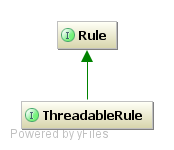
\includegraphics[scale=.4]{RuleCD}
\caption{Rule UML}
\label{UML:rule}
\end{figure}
The Rule system acts as a strategy system, and is the primary plug-in
location. Rule is (somewhat obviously) a Cellular Automata Rule. ThreadedRule is
a empty shell on top of Rule, and only exists to allow the framework to detect
if the Rule is threadable. It isn't reccomended to use it in most cases, unless
you really know what you are doing with multithreaded programming.
\subsection{Runners}
\begin{figure}[H]
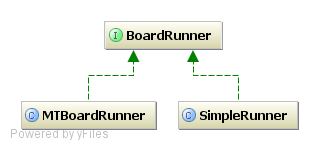
\includegraphics[scale=.4]{RunnerCD}
\caption{Runner UML}
\label{UML:runner}
\end{figure} 
The runner system is the execution system for Rules. Each runner takes a Rule
and a Board, and executes the Rule onto a board. The runner system also serves
as strategy, as it provides different ways to run Rules. The runners provided by
default in the framework implement a single threaded and a pooled threaded
multithreaded runner. A GPU based runner is in development.


The framework also allows the addition of new runners from plugins. To enable a
runner to be used, register a new RunnerFactory with BoardRunnerRepository, and
that should be that.
\subsection{Loaders}
\begin{figure}[H]
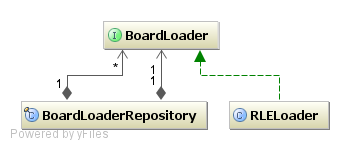
\includegraphics[scale=.4]{LoaderCD}
\caption{Loader UML}
\label{UML:loader}
\end{figure}
Loaders are used by the framework to import file formats into the board format
used by the framework. A loader is given a stream from the file and returns a
EditableBoard. Loaders are not called directly from client code, rather they are
added to the singleton BoardLoaderRepository, which is then called with a path
to a file. BoardLoaderManager then uses the loader as a strategy to parse the
file and returns the created Board.
\subsection{Views}
\begin{figure}[H]
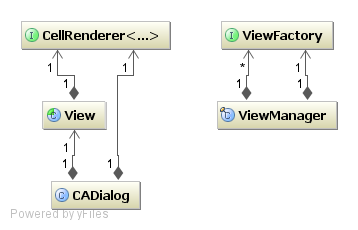
\includegraphics[scale=.4]{RendererCD}
\caption{Renderer UML}
\label{UML:renderer}
\end{figure}
The framework uses views to display boards into its window. A View takes a
instance of a CellRenderer which is then called on the cells on the board. The
rule has a reference to the View, and calls the view to render the board to the
screen.
\subsection{CellularAutomata}
\begin{figure}[H]
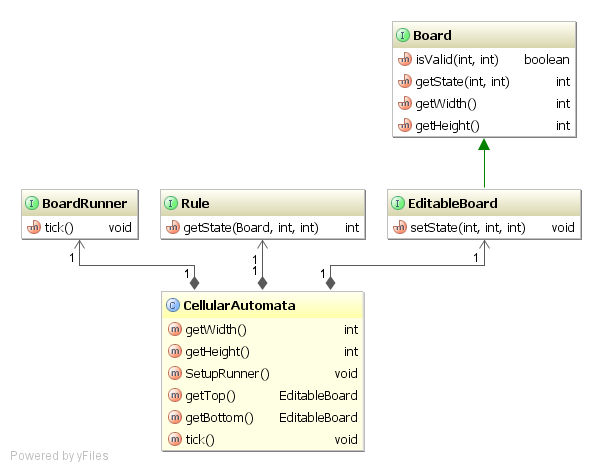
\includegraphics[scale=.4]{CellularAutomataCD}
\caption{CellularAutomata UML}
\label{UML:ca}
\end{figure}
The CellularAutomata class is the ``glue'' that holds the application toghether.
It contains the boards and calls the Runners, and provides a basic external
interface to clients.
\end{document}